\section{Introduction}
%Large language models (LLMs) \citep{brown2020language,touvron2023llama,dubey2024llama} have demonstrated remarkable capabilities, including text comprehension \citep{devlin2018bert}, generation \citep{radford2019language,goyal2020evaluating,roziere2023code}, and reasoning \citep{raffel2020exploring,wei2022chain}. A significant proportion of LLMs research focuses on external behaviors, such as task-based evaluations \citep{srivastava2022beyond,bubeck2023sparks} and designing prompts to enhance performance \citep{liu2021generated,wang2022self}. However, the inner mechanisms of LLMs remain largely unexplored, with ongoing concerns about the validity of their interpretability \citep{ghorbani2019interpretation,wen2024transformers}, and the theoretical understanding of transformers \citep{vaswani2017attention}, the core components of LLMs, is still limited.

Recent analyses of transformer-based open-source large language models (LLMs), such as GPT-2 \citep{radford2019language}, Llama-2 \citep{touvron2023llama}, Llama-3 \citep{dubey2024llama}, Mixtral \citep{jiang2023mistral}, Pythia \citep{biderman2023pythia}, and OLMo \citep{groeneveld2024olmo}, have revealed several intriguing phenomena: 
\begin{itemize}[leftmargin=2em]
\setlength\itemsep{0pt}
\item \textbf{Attention sinks} \citep{xiao2023efficient}: In many attention heads, the initial token consistently attracts a large proportion of attention weights. In certain LLMs, other special tokens, such as the delimiter token, also draw significant attention. We refer to these as \textit{sink tokens}. 
\item \textbf{Value state drains} \citep{guo2024attention}: The value states of sink tokens are consistently much smaller than those of other tokens. 
\item \textbf{Residual state peaks} \citep{sun2024massive}: The intermediate representations of sink tokens, excluding those from the first and last layers, exhibit a significantly larger norm than other tokens.
\end{itemize}
These phenomena often appear simultaneously, and we collectively refer to them as the \textbf{extreme-token phenomena}. Figure \ref{figure:extreme-token} illustrates these phenomena using a fixed prompt: ``\bos~Summer is warm. Winter is cold.'' in Llama-3.1-8B-Base, where the first token, \bos, the beginning-of-sentence token, serves as the sink token. We note that the first token does not have to be \bos~to function as a sink token, as in GPT-2, where other tokens, being the initial token, can also serve this role. Furthermore, in models like Llama-2, a delimiter token can also act as the sink token. Despite the consistency of these observations, no prior work has provided a satisfying explanation for the mechanisms behind these phenomena. As a tentative explanation, \citet{xiao2023efficient} suggested that models tend to dump unnecessary attention values to specific tokens. 

This work aims to demystify the extreme-token phenomena in LLMs. We show that the extreme-token phenomena are manifestations of the \textit{active-dormant mechanism} of attention heads. We support this claim through studies on simplified transformer architectures and tasks, a dynamical theory of simplified models, and experiments on pre-trained LLMs. Our contributions are as follows: 
\begin{enumerate}[leftmargin=2em]
\setlength\itemsep{0pt}
\item In \Cref{sec:bb_task}, we train one-to-three-layer transformers on the \textit{Bigram-Backcopy} (BB) task, which also exhibits extreme-token phenomena similar to those observed in LLMs. We show that attention sinks and value-state drains are driven by the \activedormant~mechanism. Both theoretically and empirically, we demonstrate that the mutual reinforcement dynamics underpin the extreme-token phenomena: attention sinks and value-state drains reinforce each other, leading to a stable phase where all query tokens produce identical attention logits for the keys of extreme tokens. Empirical evidence further shows that residual state peaks result from the interaction between this mutual reinforcement mechanism and Adam. 
\item In \Cref{sec:llm}, we demonstrate the \textit{\activedormant}~mechanism in LLMs by identifying an interpretable active-dormant head (Layer 16, Head 25 in Llama 2-7B-Base \citep{touvron2023llama}), confirmed through causal intervention analyses. We also discover circuits in LLMs related to extreme tokens that partially align with models trained on the BB task. Examining the dynamics of OLMo-7B-0424 \citep{groeneveld2024olmo}, we observe the same mutual reinforcement mechanism and stable phase, consistent with predictions from the BB task. 
\item Through causal interventions, we isolate the extreme-token phenomena to architecture and optimization strategy. Specifically, we show that replacing SoftMax with ReLU activations in attention heads can eliminate extreme-token phenomena in the BB task, and switching from Adam to SGD removes the residual-state peak phenomenon in the BB task. Our work demonstrates potential classes of modifications to mitigate extreme-token phenomena in LLMs. %\tianyu{I still feel that this looks not so strong.} %\DP{The phrasing should be like: We conclusively demonstrate that the extreme-token phenomenon is a property of the specific architecture and optimization procedure, and show this via two ablation tests in the BB task: replacing SoftMax with ReLU in the attention mechanism and switching Adam to SGD. Our work demonstrates potential classes of mechanisms to mitigate extreme-token phenomena in LLMs.}
\end{enumerate}

\yub{We release our code at the following anonymous repo: XXX.}
% \begin{enumerate}[leftmargin=2em]
% \setlength\itemsep{0pt}
% \item We design the \textit{Bigram-Backcopy} (BB) task, train one-to-three layer transformers, and recapitulate the extreme token phenomena, offering a framework for understanding the \activedormant. Both theoretically and empirically, we demonstrate the mutual reinforcement dynamics of the extreme token phenomena. Our key finding is that the attention sinks and value state drains reinforce each other in the dynamics, leading to the stable phase consists of identical attention logits from all query tokens to the key of extreme tokens. With empirical evidence, we demonstrate that residual state peaks result from the interaction of this mutual reinforcement mechanism with Adam.
% \item Extending the findings from small models to LLMs, we first discover an interpretable active-dormant head (Layer 16 Head 25 in Llama 2-7B-Base \citep{touvron2023llama}), verified through causal interventions. We also discover circuits in LLMs for the extreme tokens that partially match the models trained for the BB task. We inspect the dynamics of OLMo-7B-0424 \citep{groeneveld2024olmo}, identifying the same mutual reinforcement mechanism and stable phase, consistent with predictions from the BB task analysis.
% \item As broader implications, we demonstrate potential design choices to mitigate extreme-token phenomena in LLMs. we propose two methods to eliminate the extreme-token phenomena based on the discovered mechanisms: replacing SoftMax with ReLU activations in attention heads and switching Adam to SGD, both verified in the BB task. \tianyu{I still feel that this looks not so strong.} \DP{The phrasing should be like: We conclusively demonstrate that the extreme-token phenomenon is a property of the specific architecture and optimization procedure, and show this via two ablation tests in the BB task: replacing SoftMax with ReLU in the attention mechanism and switching Adam to SGD. Our work demonstrates potential classes of mechanisms to mitigate extreme-token phenomena in LLMs.}
% \end{enumerate}



\begin{figure}[t]
  \centering
  \begin{subfigure}[t]{0.32\textwidth}
      \centering 
      \caption{\small Attention weights at L24.}
      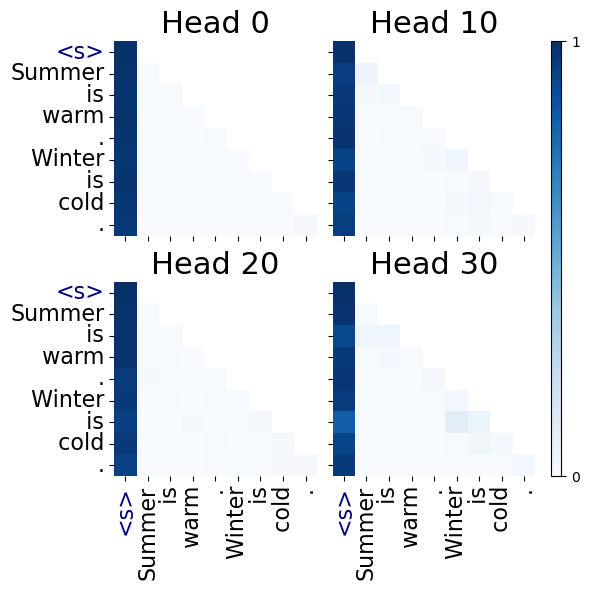
\includegraphics[width=\textwidth]{Figures/demo_attn_sink.png}
      \label{fig:attention_sinks_wide_random}
  \end{subfigure}
  \hfill
  % \begin{subfigure}[t]{0.32\textwidth}
  %     \centering 
  %     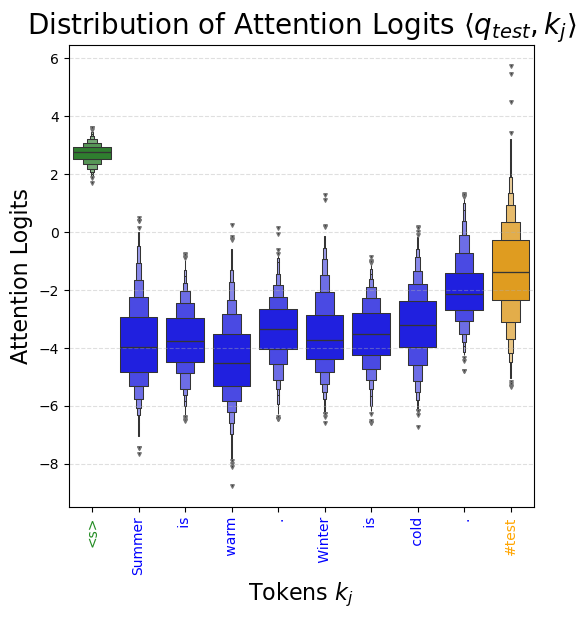
\includegraphics[width=\textwidth]{Figures/attn_logits_random_tokens.png}
  %     \caption{\small Attention logits \(\langle \bm{q}_{\mathrm{test}}, \bm{k}_{j}\rangle\).}
  %     \label{fig:attention_logits_random}
  % \end{subfigure}
  \begin{subfigure}[t]{0.3\textwidth}
      \centering 
      \caption{\small Norms of residual states.}
      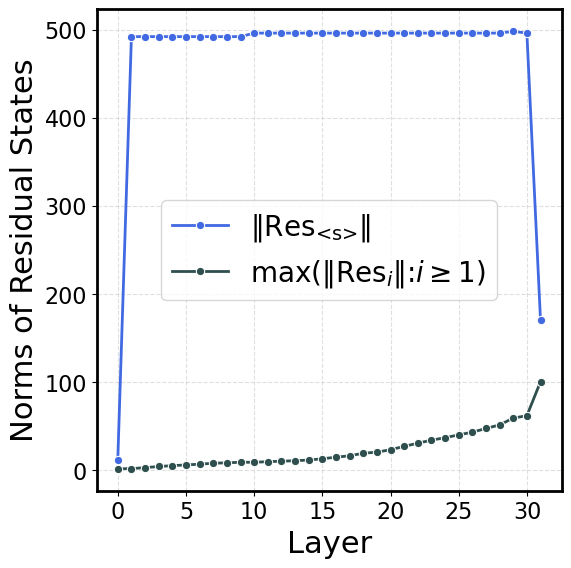
\includegraphics[width=\textwidth]{Figures/residual_norms.png}
      \label{fig:token_norms_massive}
  \end{subfigure}
  \hfill
  \begin{subfigure}[t]{0.3\textwidth}
      \centering 
      \caption{\small Norms of value states.}
      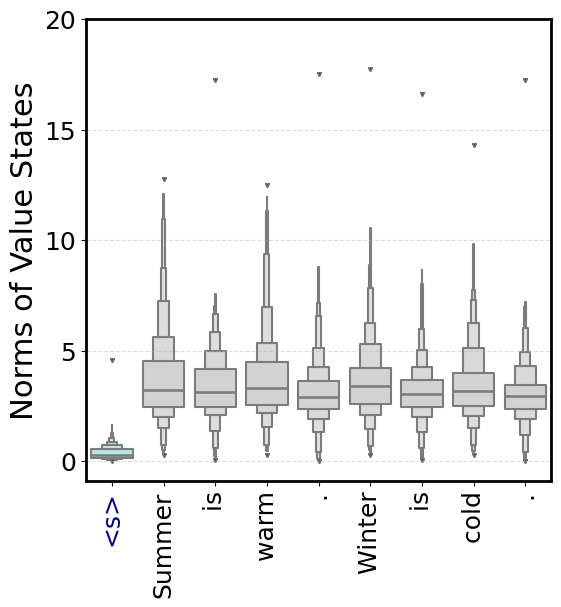
\includegraphics[width=\textwidth]{Figures/value_state_norms.png}
      \label{fig:value_norms_zeroed}
  \end{subfigure}
  
  % \begin{minipage}{0.33\textwidth}
  %     \centering
  %     \subcaption{\small Attention logits}
  %     \label{fig:circuit-attn-logits}
  %     \vspace{-.2em}
  %     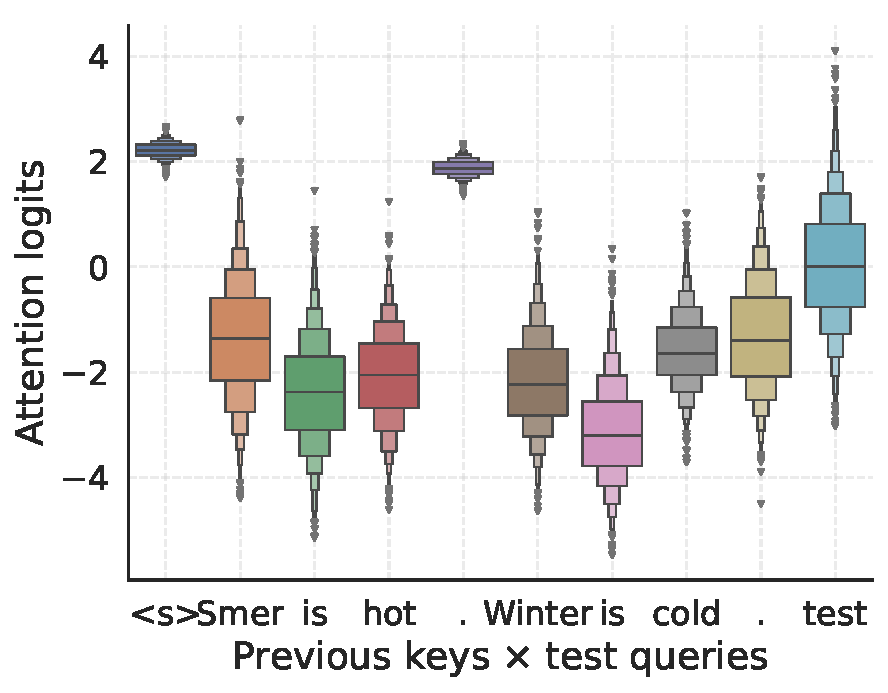
\includegraphics[width=\linewidth]{Figures/figures_circuit/logits.pdf}
  % \end{minipage}~
  % % \hspace{-1em}
  % \begin{minipage}{0.33\textwidth}
  %     \centering
  %     \subcaption{\small Residual states norm}
  %     \label{fig:circuit-massive-norm}
  %     \vspace{-.2em}
  %     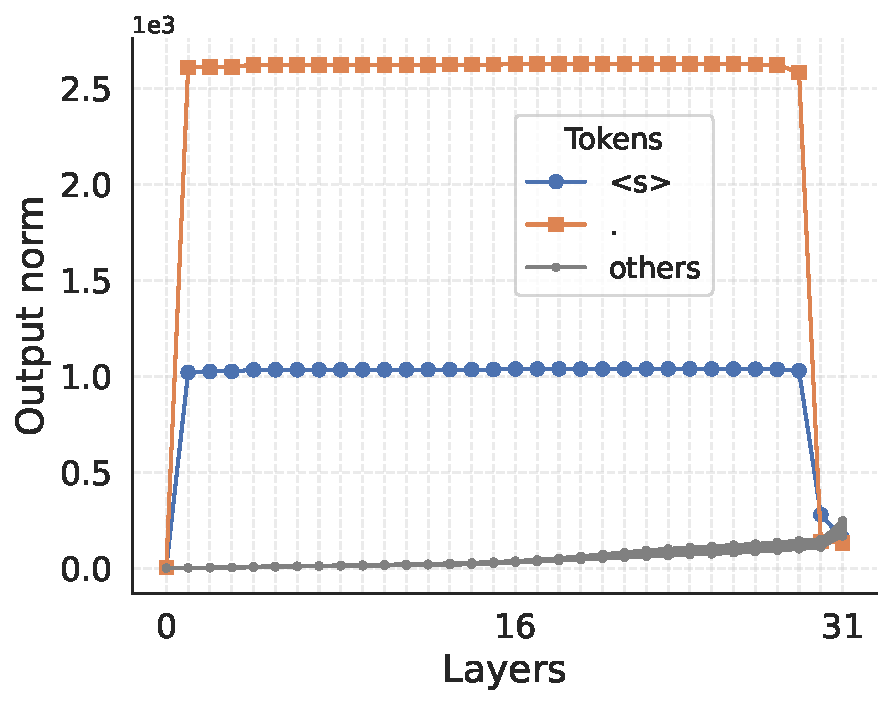
\includegraphics[width=\linewidth]{Figures/figures_circuit/massive.pdf}
  % \end{minipage}
  % \hspace{-1em}
  % \begin{minipage}{0.33\textwidth}
  %     \centering
  %     \subcaption{\small Value states norm}
  %     \label{fig:circuit-value-norm}
  %     \vspace{-.2em}
  %     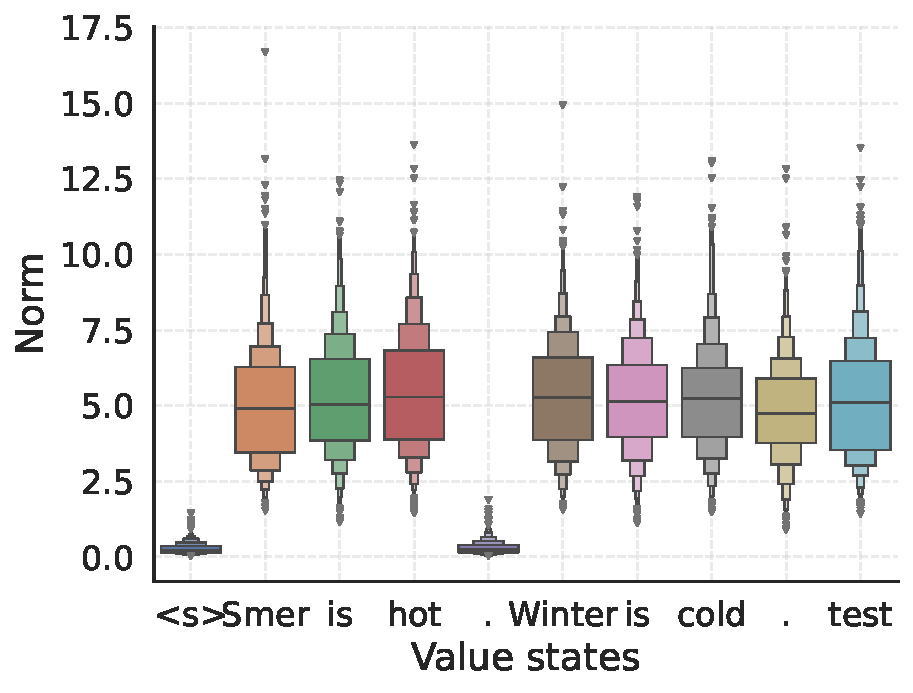
\includegraphics[width=\linewidth]{Figures/figures_circuit/values.pdf}
  % \end{minipage}
  \vspace{-2em}
  \caption{\small \textbf{Extreme-token phenomena in Llama 3.1-8B-Base.}
  %\tianyu{bigger text size; remove all labels in the middle of fig (a); notations; thicker lines;  remove all test tokens. backup plan: include more heads} 
  We evaluate the sentence ``\bos~Summer is warm. Winter is cold.'' on the Llama 3.1-8B-Base model. \textit{Left (a):} The value of the attention weights across multiple heads at Layer 24. We demonstrate that there are \textit{attention sinks}: the key state associated with the \bos{} token attracts the most attention from query states in these (and most) heads. 
 % Figure \ref{fig:attention_logits_random} displays the distribution of attention logits \(\langle \bm{q}_{\mathrm{test}}, \bm{k}_{i}\rangle\) across all heads and test tokens at Layer 24. %\sm{which head?}. 
  %The logits for the \bos~token 
  %~and the first \delim~
  %are concentrated at large values, while those for other tokens are smaller and fluctuate across different random test tokens. 
  \textit{Middle (b):} The norm of the (residual stream) hidden states, measured at the output of each layer. We observe a \textit{residual state peak} phenomenon: the \bos~token's residual states have significantly larger norms than those of other tokens from layers 1 to 30. 
  %\sm{1 to 30?} \DP{Yes, 1-30}
  \textit{Right (c):} The distribution of the norms of value states corresponding to each token at all layers 
  %\sm{all or 1-30?} \DP{all}
  and all heads. We observe the \textit{value state drain} phenomenon: across many attention heads, the value state of the \bos~token is much smaller than those of other tokens on average. %\sm{Edit figure}
  }
  \label{figure:extreme-token}
  \vspace{-1em}
\end{figure}



% \yub{LLMs...}~\yub{a sophisticated but extremely powerful system}~\yub{however are there any structural biases?}

% \yub{some recent works identify an intruiging phenomenon in trained LLMs.}~\yub{describe the sink token phenomenon.}~\yub{two features: massive in norm, and caused by massive in specific entries~\citep{sun2024massive}, and attract attention scores (give rigorous description)~\citep{xiao2023efficient,darcet2023vision}}~\yub{Has been used in applications such as Streaming LLM generation~\citep{xiao2023efficient,han2023lm}.}

% Despite the intriguing findings, the understanding is still~\yub{at a surface level}, with many questions unanswered.~\yub{1. what tokens get to be sink tokens, and how is this process related to the position of the tokens in the sequence?}~\yub{second delimiter thing...}~\yub{2. is attention concentration phenomenon a consequence of the massive norms?}~\yub{3. Does attention concentration imply that non-sink tokens are not important to the final attention output?}


% In this work, we provide a more in-depth understanding on how sink tokens arise and take effect in trained LLMs. Our contributions can be summarized as follows.
% \begin{itemize}
%     \item BLAH.
% \end{itemize}



\subsection{Notation}
We denote the SoftMax attention layer with a causal mask as $\attn$, the MLP layer as $\mlp$, and the transformer block as $\TF$. The query, key, value states, and residuals of a token $\tok$ are represented as $\query_\tok$, $\key_\tok$, $\val_\tok$, and $\res_\tok$, respectively, with the specific layer and head indicated in context. We use \bos~to refer to the "Beginning of Sequence" (bos) token. Throughout the paper, we employ zero-indexing (i.e., attention head and layer indices start from 0 rather than 1) for consistency between code and writing. 
